% Detail retained for questions after the main talk.

\sectionframe{Appendix. Data and Descriptive Detail}

\begin{frame}{Roadmap}
  \begin{enumerate}
    \item Motivation and data.
    \item Descriptive statistics.
    \item Conditional firm-size wage premium.
    \item Dynamics and elasticities.
    \item Illustrative income scenarios.
    \item Interpretation and policy implications.
  \end{enumerate}
\end{frame}

\begin{frame}{Main Results}
  \begin{columns}[T,totalwidth=\textwidth]
    \begin{column}{0.49\textwidth}
      \vspace{0.25cm}
      \begin{itemize}
        \item Large firms pay more than solo work in the raw data.
        \item The relationship survives controls for observable characteristics.
        \item The 101+ premium vs solo workers is 37\% among informal and 17\% among formal workers.
      \end{itemize}
    \end{column}
    \begin{column}{0.49\textwidth}
      \vspace{0.25cm}
      \begin{itemize}
        \item Among salaried workers, the formal and informal 101+/solo premiums are both about 21\%.
        \item Assigning everyone to formal 101+ jobs implies 25.9\% higher total predicted labor income in the full sample and 12.3\% in the salaried workers sample.
        \item The premium does not prove causality or misallocation by itself.
      \end{itemize}
    \end{column}
  \end{columns}
\end{frame}

\begin{frame}{Why Firm Size Matters}
  \idea{Firm size captures a visible dimension of the productive structure.}

  \vspace{0.35cm}
  \begin{itemize}
    \item In Colombia, a large share of employment is concentrated in own-account work and micro-firms.
    \item If hourly pay is systematically higher in larger firms, the firm-size distribution matters for wage inequality.
    \item The relationship can also be informative about frictions: barriers to growth, formalization, market access, or worker reallocation toward better firms.
  \end{itemize}
\end{frame}

\begin{frame}{Data}
  \idea{We use GEIH observations for workers who report the size of the unit in which they work.}

  \vspace{0.3cm}
  \begin{itemize}
    \item Source: Gran Encuesta Integrada de Hogares, DANE.
    \item Period: 2008--2019 and 2021--2025.
    \item We exclude 2020 because of pandemic-related data limitations.
    \item Sample: 5.43 million observations across repeated cross-sections, covering all twelve months of each included year.
    \item Ages 15--120, positive main-job income, valid main-job hours, and complete controls.
    \item Income excludes earnings from secondary jobs. Pension recipients are excluded from the formal-informal comparison.
  \end{itemize}
\end{frame}

\begin{frame}{Main Variables}
  \begin{columns}[T,totalwidth=\textwidth]
    \begin{column}{0.48\textwidth}
      \idea{Hourly pay}
      \vspace{0.25cm}
      \[
        w_{it} =
        \frac{12 \times MonthlyIncome_{it}}
        {52 \times WeeklyHours_{it}}
        \times
        \frac{CPI_{2025}}{CPI_t}
      \]
      \vspace{0.1cm}
      {\small Income and hours refer to the main job. Real hourly labor income is in constant 2025 Colombian pesos.}
    \end{column}
    \begin{column}{0.48\textwidth}
      \idea{Firm size}
      \vspace{0.25cm}
      \begin{itemize}
        \item Solo
        \item 2--3, 4--5, 6--10
        \item 11--19, 20--30, 31--50, 51--100
        \item 101+
      \end{itemize}
      {\small We combine 101--200 and 201+ into 101+ to match earlier questionnaires.}
    \end{column}
  \end{columns}
\end{frame}

\begin{frame}{Firm Size and Status in Employment}
  \idea{Solo work describes the size of the reported unit, not the worker's status in employment.}
  \vspace{0.3cm}
  \begin{itemize}
    \item A household's sole domestic employee is a solo worker, but not an own-account worker.
    \item Own-account workers may report larger units when working with partners, unpaid family helpers, or as contractors.
    \item GEIH assigns state contractors to 101+ despite their own-account status.
    \item Status in employment is recorded separately and included as a control.
  \end{itemize}
  %\source{Paper Section 2. DANE's GEIH collection manual (2025), pp. 89--90 and 115.}
\end{frame}

\begin{frame}{Formality}
  \idea{We define formality through pension contribution.}

  \vspace{0.35cm}
  \begin{itemize}
    \item A worker is formal if the worker contributes to pensions.
    \item A worker is informal if the worker does not contribute to pensions.
    \item Employed pension recipients are excluded from the formal-informal comparisons.
    \item This is a worker-level measure of their formality status, not a measure of the firm's formality status.
    \item The definition does not use firm size.
  \end{itemize}
\end{frame}

\begin{frame}{The Size Gap Relative to Other Wage Gaps}
  \idea{The raw firm-size gap is comparable to the formal-informal gap and smaller than the largest education and sector gaps.}

  \vspace{0.25cm}
  \begin{center}
  \scriptsize
  \setlength{\tabcolsep}{3pt}
  \begin{tabular}{p{0.38\textwidth}rp{0.30\textwidth}}
    \toprule
    2025 comparison & Ratio between extremes & Reading \\
    \midrule
    Women / men & 1.02 & Small gap in means \\
    Formal / informal & 2.43 & Very large gap \\
    Higher education / preschool or less & 4.06 & Larger than the size gap \\
    Information and communication / agriculture & 3.68 & Very large sector gap \\
    101+ / solo & 2.59 & Large firm-size gap \\
    \bottomrule
  \end{tabular}
  \end{center}

  \source{Ratios are based on real hourly labor income in constant 2025 pesos.}
\end{frame}

\begin{frame}{How to Read the U-Shape among Formal Workers}
  \idea{Formal solo work includes relatively well-paid independent professionals, alongside other workers.}

  \vspace{0.35cm}
  \begin{itemize}
    \item In 2025, 82.1\% of formal solo workers were own-account workers and 16.2\% were domestic workers.
    \item 50.8\% had higher education.
    \item Among those with higher education, 95.5\% were own-account workers, with legal and accounting services among the most common activities.
    \item Mean hourly income was 21,333 pesos with higher education, versus 9,835 without it.
  \end{itemize}
  \source{Paper Table~\paperref{tab:formal-worker-profile-2025} and accompanying text. All figures refer to formal solo workers in 2025. Income in 2025 pesos.}
\end{frame}

\begin{frame}{The Raw Premium Appears within Men and Women}
  \centering
  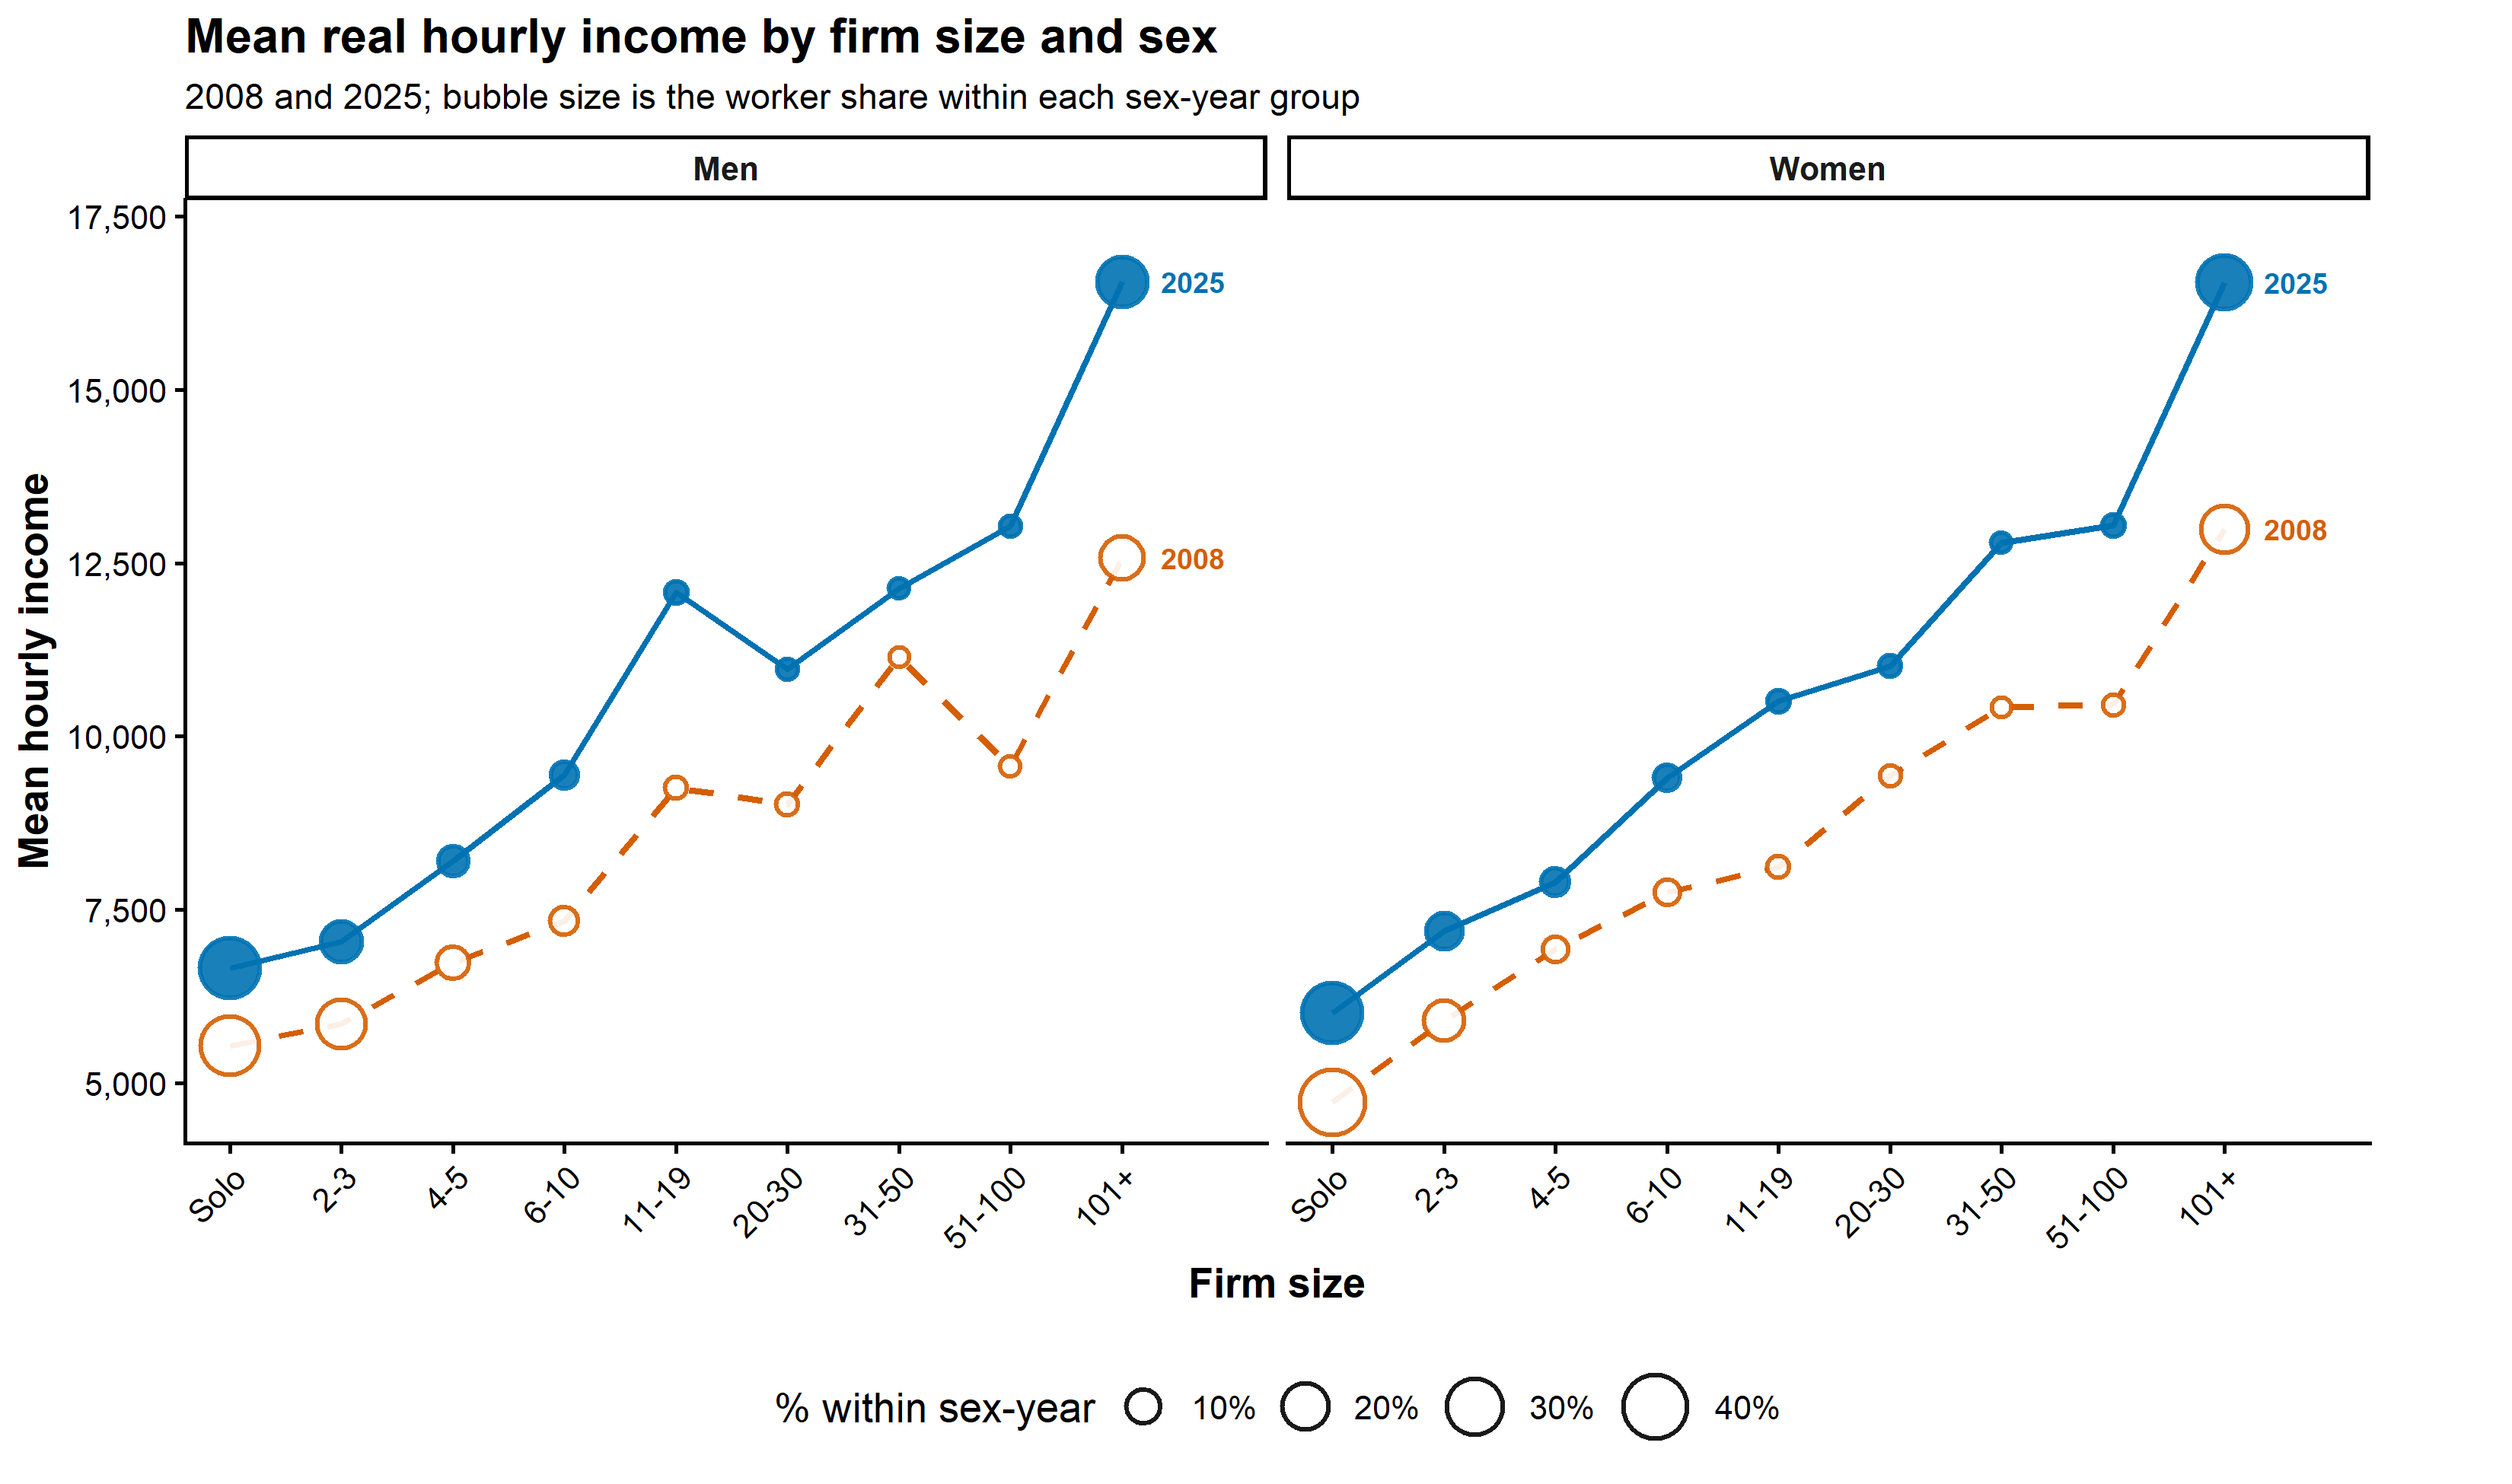
\includegraphics[width=0.94\textwidth,height=0.79\textheight,keepaspectratio]{fig70_en.png}

  \source{The sex gap within each size category is small relative to the gap between solo work and large-firm employment.}
\end{frame}

\begin{frame}{The Raw Premium Appears within Each Education Group}
  \centering
  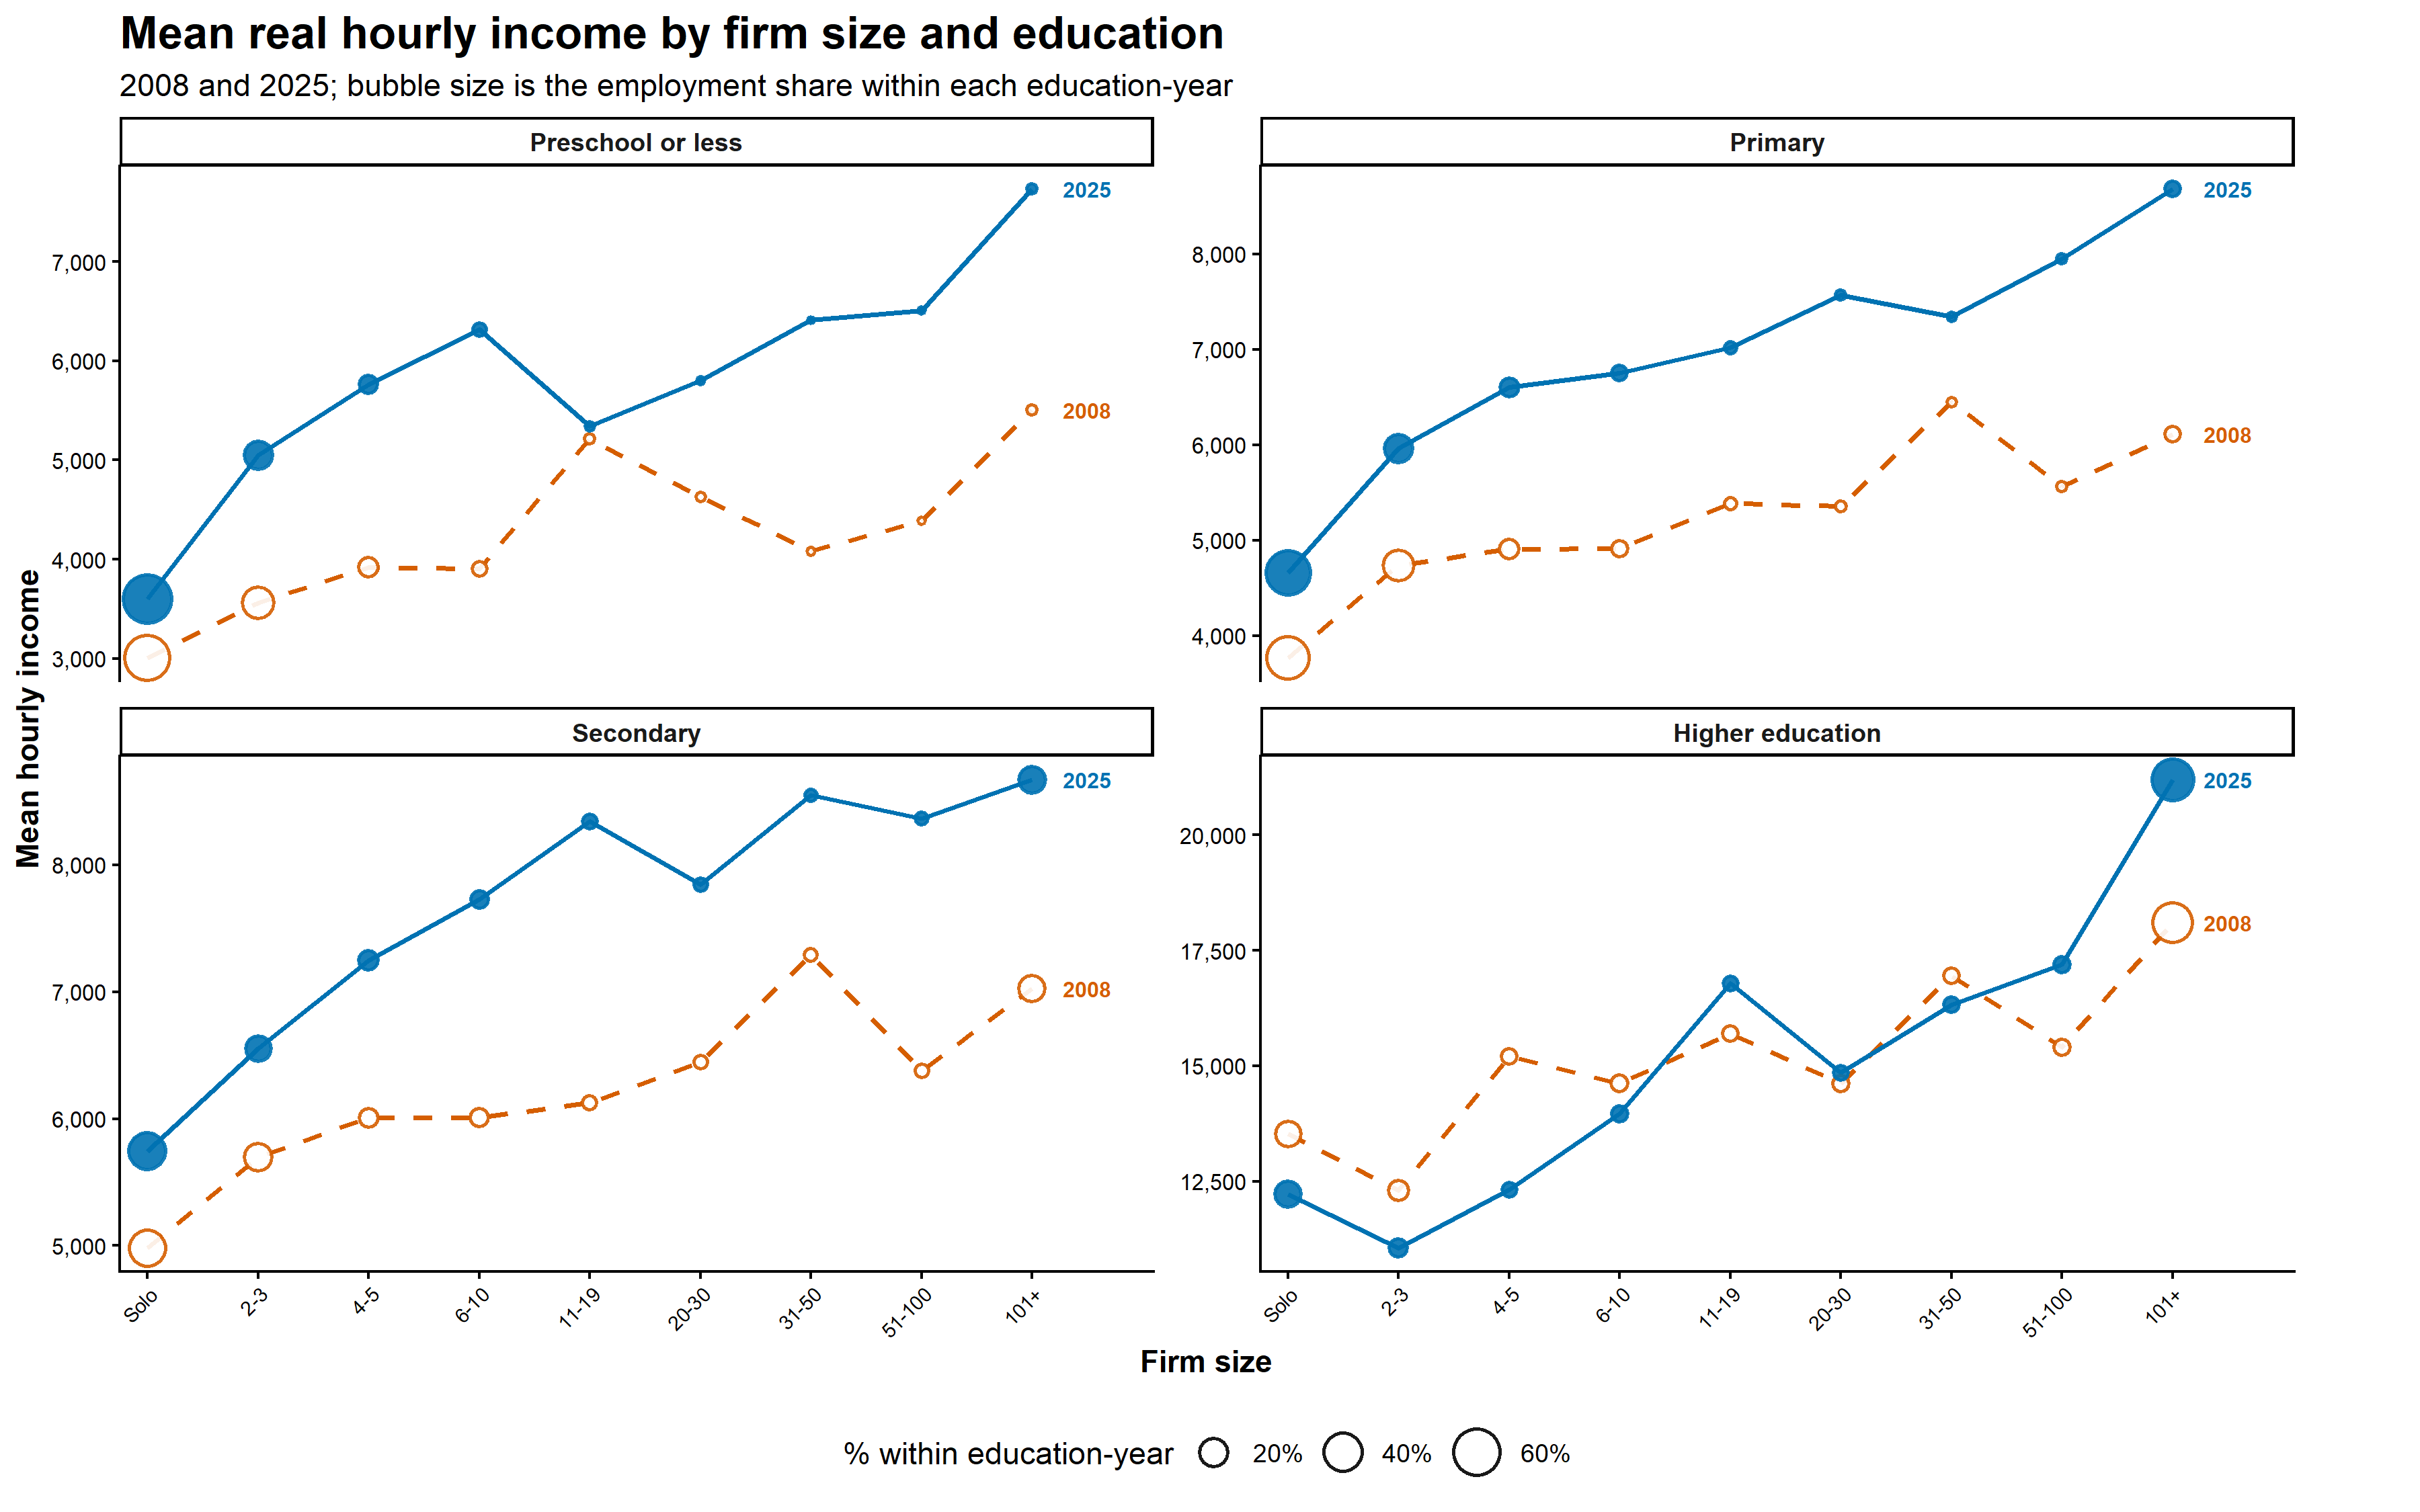
\includegraphics[width=0.96\textwidth,height=0.79\textheight,keepaspectratio]{fig72_en.png}

  \source{The 101+/solo ratio was 2.1 for preschool or less, 1.9 for primary, 1.5 for secondary, and 1.7 for higher education.}
\end{frame}

\begin{frame}{Firm-Size Wage Gaps by Sector (1/2)}
  \centering
  {\scriptsize Mean real hourly income in 2025 pesos\par}
  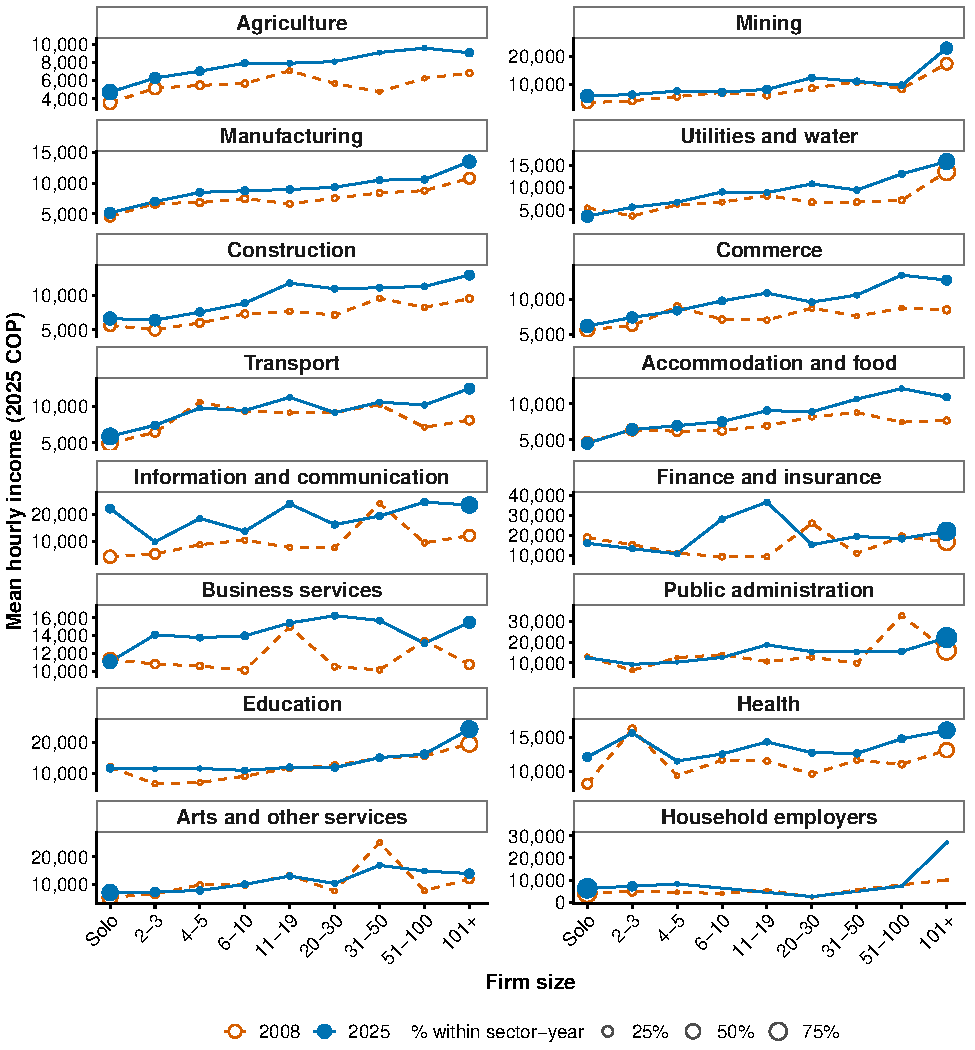
\includegraphics[width=0.76\textwidth,trim=13bp 285bp 0 0,clip]{fig71_en.pdf}
  \par
  % Repeat the common size axis and bubble legend below the upper four rows.
  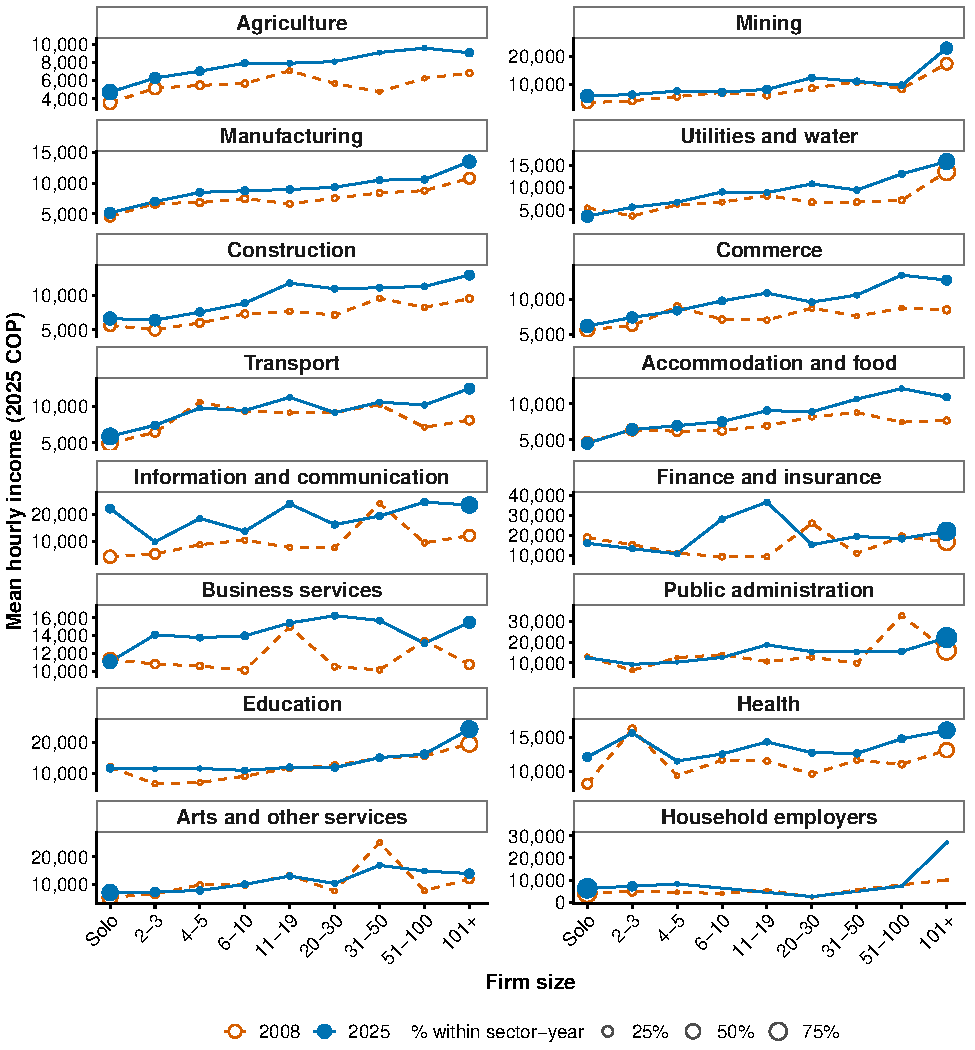
\includegraphics[width=0.76\textwidth,trim=13bp 0 0 437bp,clip]{fig71_en.pdf}
  \source{Paper Figure~\paperref{fig:income-sector-comparison}. The 101+/solo ratio in agriculture declined from about 2.5 to 2.0. In manufacturing, it rose from 2.46 to 2.68.}
\end{frame}

\begin{frame}{Firm-Size Wage Gaps by Sector (2/2)}
  \centering
  {\scriptsize Mean real hourly income in 2025 pesos\par}
  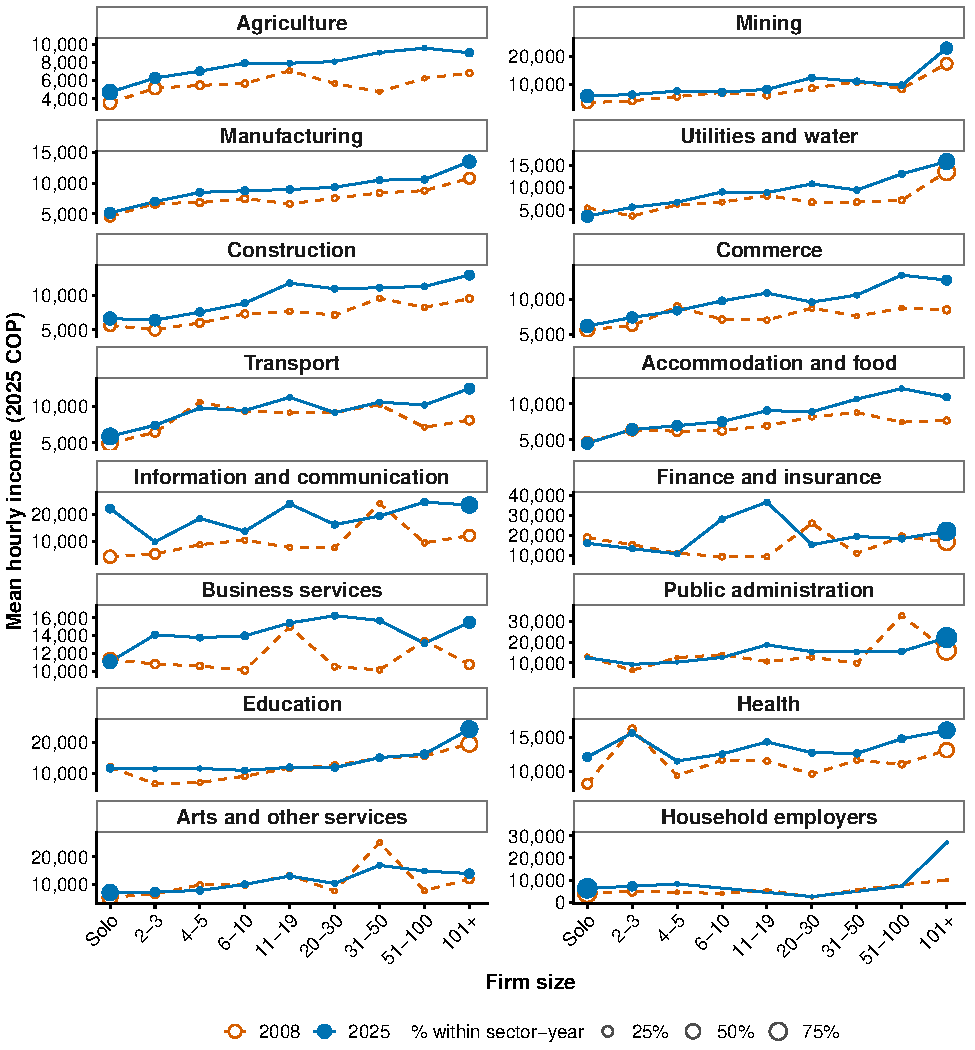
\includegraphics[width=0.76\textwidth,trim=13bp 0 0 219bp,clip]{fig71_en.pdf}
  \source{Paper Figure~\paperref{fig:income-sector-comparison}. The 101+/solo advantage appears in 14 of 16 sectors in both years and all 16 in 2025. It need not increase at every size category.}
\end{frame}

\sectionframe{Appendix. Specifications and Additional Results}

\begin{frame}{Start with the Simplest Specification}
  \[
  \ln w_{ist}=\alpha+\sum_{g\ne g_0}\beta_g D_{ig}+\varepsilon_{ist}.
  \]
  \begin{enumerate}
    \item Start with firm-size indicators alone.
    \item Add sector-year fixed effects.
    \item Add sex, age, age squared, and education.
    \item Add formality as a level control.
  \end{enumerate}
  \vspace{0.2cm}
  \idea{This sequence still imposes the same size coefficients on formal and informal workers.}
  %\source{Paper Table~\paperref{tab:firm-size-wage-premium-regressions}. $g_0$ denotes solo work. Column (4) estimates Equation~(\paperref{eq:common-premium}). All columns use the same 5,426,316 observations.}
\end{frame}

\begin{frame}{Then Add Geography and Status in Employment}
  \centering\begingroup\fontsize{8.5}{10}\selectfont
  \setlength{\tabcolsep}{4pt}
  \begin{adjustbox}{max width=\textwidth,max totalheight=0.68\textheight}
    \begin{tabular}{lcccc}
\toprule
    & \multicolumn{4}{c}{Dependent variable: log real hourly labor income} \\
    \cmidrule(lr){2-5}
    & (1) & (2) & (3) & (4) \\
    \midrule
Firm size: 2-3 & 0.188*** \sereg{0.011} & 0.168*** \sereg{0.011} & 0.167*** \sereg{0.011} & 0.102*** \sereg{0.013} \\
Firm size: 4-5 & 0.307*** \sereg{0.014} & 0.277*** \sereg{0.014} & 0.273*** \sereg{0.014} & 0.225*** \sereg{0.015} \\
Firm size: 6-10 & 0.316*** \sereg{0.018} & 0.282*** \sereg{0.017} & 0.278*** \sereg{0.017} & 0.265*** \sereg{0.016} \\
Firm size: 11-19 & 0.302*** \sereg{0.018} & 0.272*** \sereg{0.017} & 0.267*** \sereg{0.017} & 0.272*** \sereg{0.015} \\
Firm size: 20-30 & 0.271*** \sereg{0.019} & 0.241*** \sereg{0.017} & 0.237*** \sereg{0.017} & 0.258*** \sereg{0.015} \\
Firm size: 31-50 & 0.271*** \sereg{0.018} & 0.245*** \sereg{0.017} & 0.240*** \sereg{0.017} & 0.263*** \sereg{0.015} \\
Firm size: 51-100 & 0.289*** \sereg{0.018} & 0.262*** \sereg{0.017} & 0.257*** \sereg{0.017} & 0.282*** \sereg{0.015} \\
Firm size: 101+ & 0.359*** \sereg{0.023} & 0.338*** \sereg{0.024} & 0.325*** \sereg{0.024} & 0.338*** \sereg{0.022} \\
\midrule
    Worker and formality controls & Yes & Yes & Yes & Yes \\
Occupational-position controls & No & No & No & Yes \\
Fixed effects & $s\times t$ & $s\times t$, $d\times t$ & $s\times d\times t$ & $s\times d\times t$ \\
Observations & 5,268,514 & 5,268,514 & 5,268,375 & 5,268,375 \\
$R^2$ & 0.386 & 0.404 & 0.414 & 0.429\\
\bottomrule\end{tabular}

  \end{adjustbox}\endgroup
  \par\vspace{0.15cm}
  {\small The final 101+/solo coefficient is 0.343, or 41.0\%. But should one size premium describe both formal and informal employment?}
  %\source{Paper Table~\paperref{tab:firm-size-local-geography-robustness}. Column (4) estimates Equation~(\paperref{eq:common-premium-geography}). SEs cluster by sector-department. Columns (3)--(4) exclude 142 singleton observations.}
\end{frame}

\begin{frame}{What the Coefficients Compare}
  \begin{center}
  \small
  \begin{tabular}{lll}
  \toprule
  Log-income comparison & Contrast & Coefficients \\
  \midrule
  Informal, size $g$ to $h$ & $\Delta^I_{g\to h}$ & $\beta_h-\beta_g$ \\
  Formal, size $g$ to $h$ & $\Delta^F_{g\to h}$ & $(\beta_h+\theta_h)-(\beta_g+\theta_g)$ \\
  Informal to formal, size $g$ & $\Delta^{I\to F}_g$ & $\phi+\theta_g$ \\
  \bottomrule
  \end{tabular}
  \end{center}
  \vspace{0.25cm}
  \begin{itemize}
    \item For each estimated contrast $\widehat\Delta$, report $100[\exp(\widehat\Delta)-1]$.
    \item These are ratios of exponentiated conditional mean log incomes, not necessarily ratios of arithmetic means.
  \end{itemize}
  %\source{Contrasts from Paper Equation~(\paperref{eq:main}). Changing the reference category leaves fitted values and pairwise comparisons unchanged.}
\end{frame}

\begin{frame}{Preferred Regression Output}
  \centering\small
  \begin{tabular}{lcc}
  \toprule
  Firm size & Informal: $\widehat\beta_g$ & Formal: $\widehat\beta_g+\widehat\theta_g$ \\
  \midrule
  2--3 & 0.112*** \sereg{0.013} & -0.075*** \sereg{0.028} \\
  4--5 & 0.257*** \sereg{0.016} & -0.023 \sereg{0.033} \\
  6--10 & 0.324*** \sereg{0.017} & 0.014 \sereg{0.034} \\
  11--19 & 0.354*** \sereg{0.018} & 0.041 \sereg{0.031} \\
  20--30 & 0.364*** \sereg{0.017} & 0.043 \sereg{0.031} \\
  31--50 & 0.363*** \sereg{0.020} & 0.064** \sereg{0.031} \\
  51--100 & 0.375*** \sereg{0.020} & 0.089*** \sereg{0.031} \\
  101+ & 0.315*** \sereg{0.019} & 0.159*** \sereg{0.037} \\
  \bottomrule
  \end{tabular}
  \par\vspace{0.25cm}
  {\small Reference: solo workers of the same formality status.}
  \regnote{Log-point contrasts, not percent premiums. Standard errors in parentheses are clustered by sector-department. * $p<0.10$, ** $p<0.05$, *** $p<0.01$.}
\end{frame}

\begin{frame}{Has the Conditional Premium Changed?}
  \small
  \begin{align*}
    \ln w_{iosdt}={}&\sum_{\tau\in\mathcal T}\mathbf{1}\{t=\tau\}
    \left[\phi_\tau F_i+\sum_{g\ne g_0}(\beta_{g\tau}+\theta_{g\tau}F_i)D_{ig}
    +X_i'\gamma_\tau+\rho_{o\tau}\right]\\
    &+\lambda_{s\times d\times t}+\varepsilon_{iosdt}.
  \end{align*}
  \begin{itemize}
    \item All size, formality, worker-control, and status-in-employment coefficients vary by year.
    \item Annual profiles come from separate yearly regressions.
    \item Test 2008--2025 changes jointly, retaining cross-year covariance within clusters.
  \end{itemize}
  \vspace{0.2cm}
  \idea{All change tests are two-sided. Widening and narrowing are both possible.}
  \source{Paper Equation~(\paperref{eq:preferred-dynamics}). $\mathcal T$ is the set of sample years. Endpoint tests are pointwise, without multiple-testing adjustment.}
\end{frame}

\begin{frame}{Adjusted Profiles in 2008 and 2025}
  \centering
  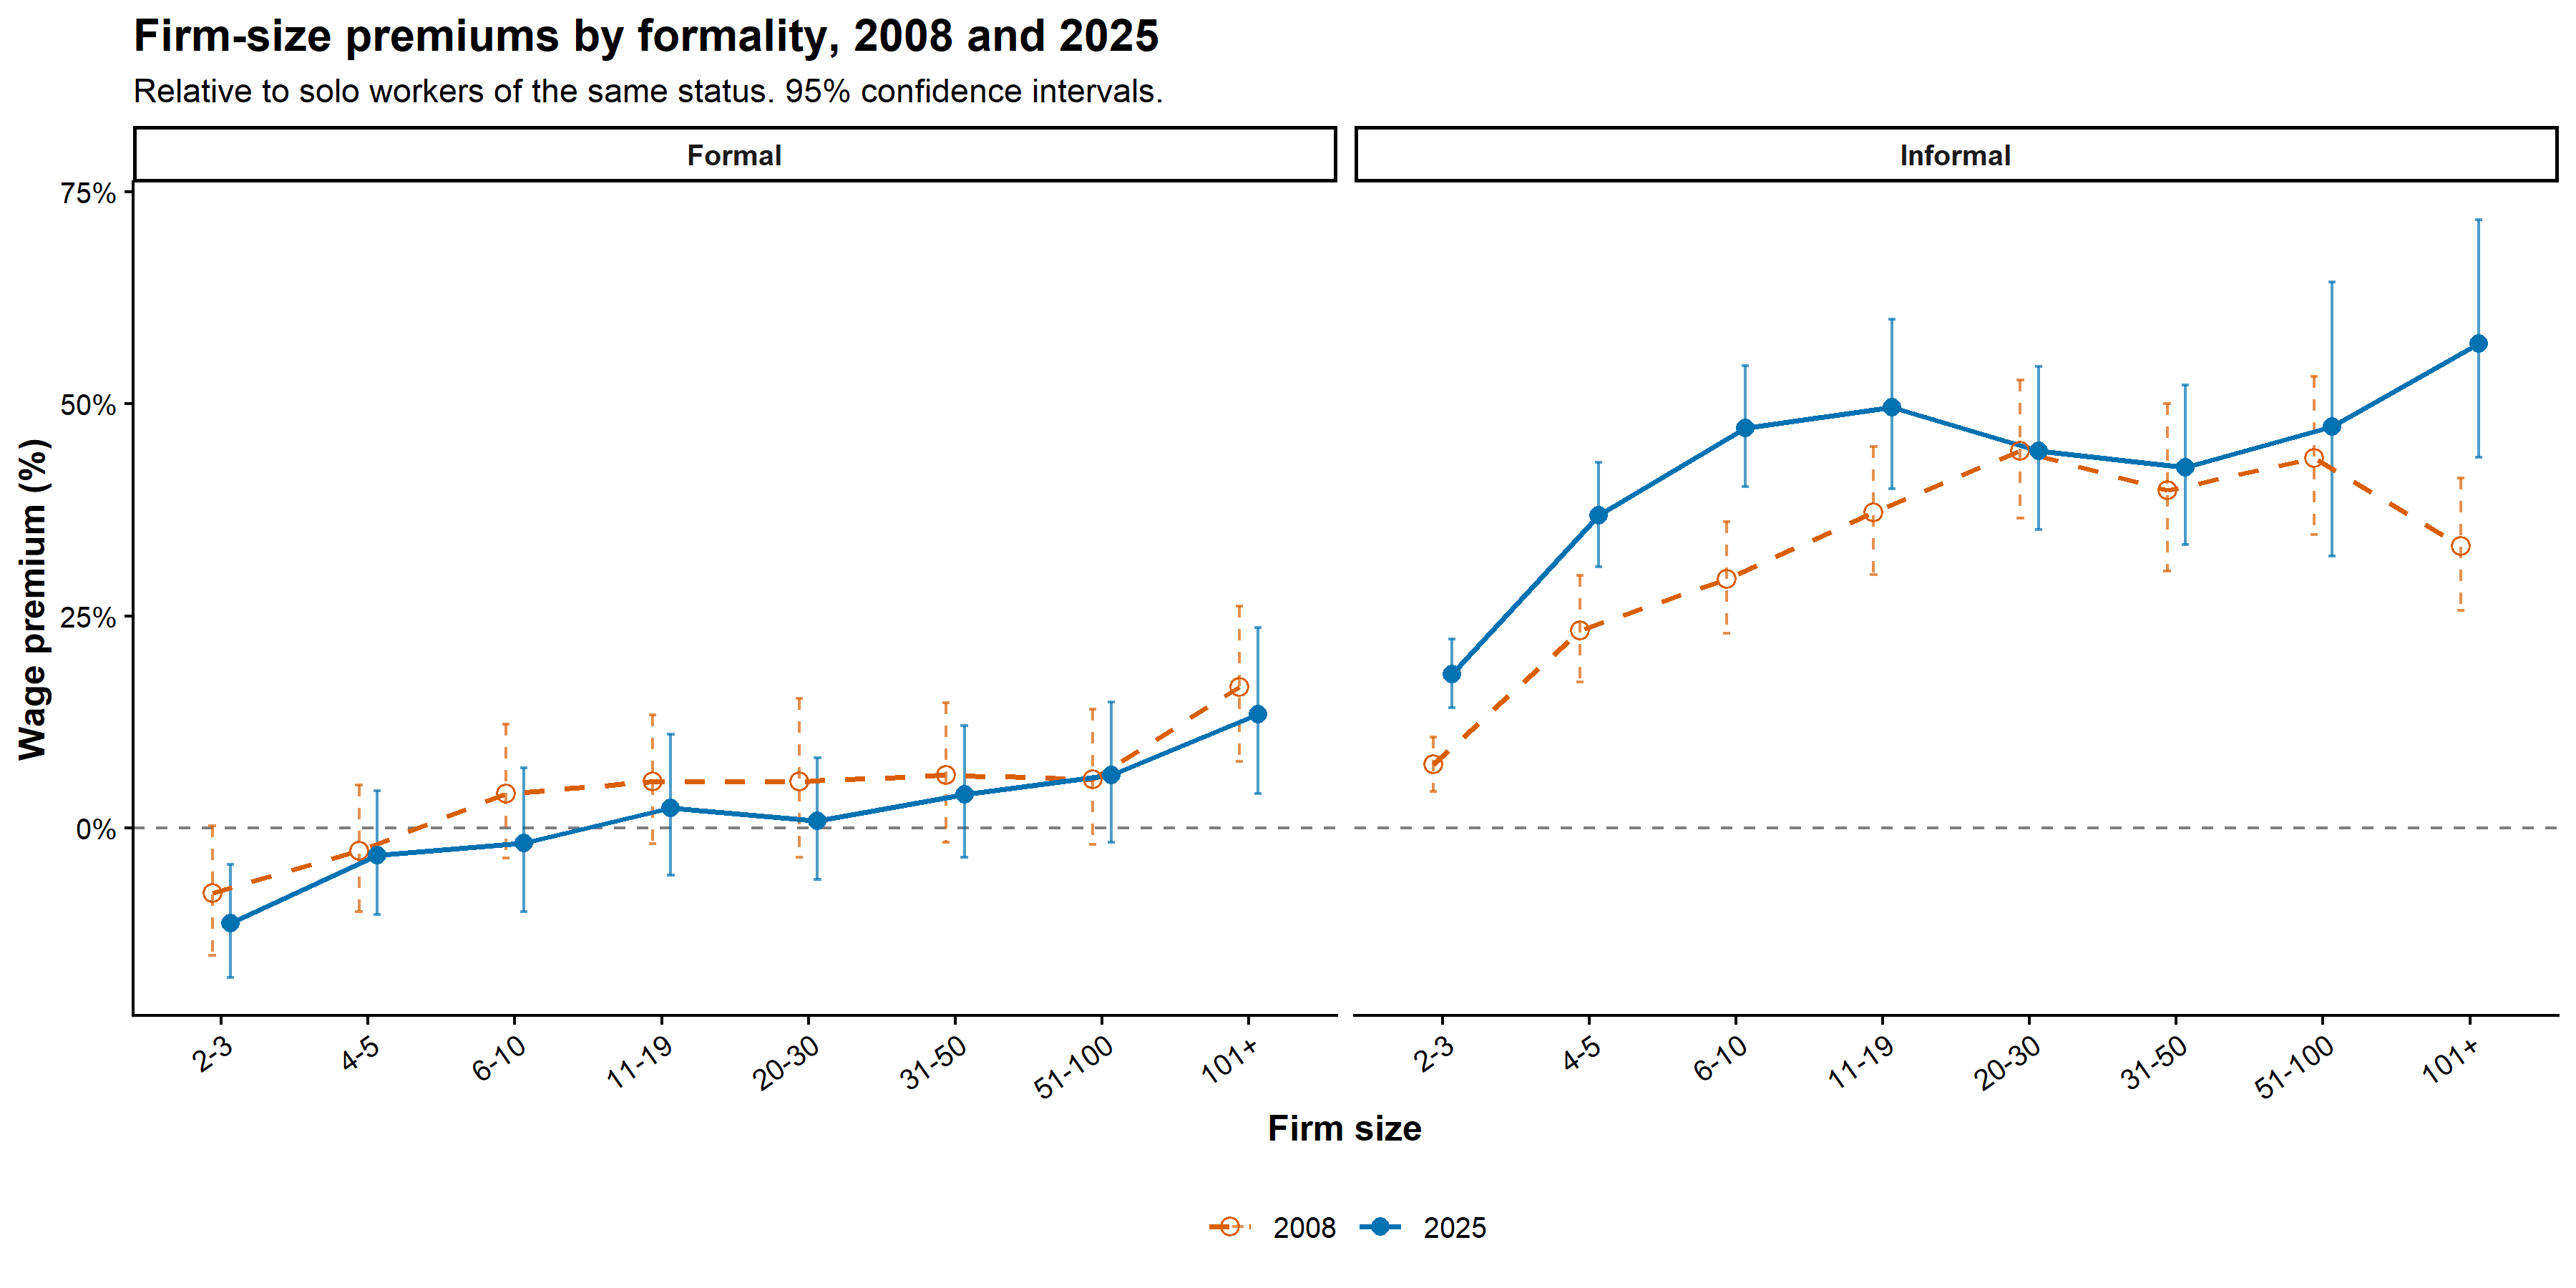
\includegraphics[width=0.98\textwidth,height=0.80\textheight,keepaspectratio]{preferred_formality_endpoints_en.png}
  \source{Paper Figure~\paperref{fig:preferred-formality-endpoints}, Equation~(\paperref{eq:preferred-dynamics}). Reference is solo work within each formality-year group. Intervals use sector-department clustering.}
\end{frame}

\begin{frame}{Contrast with Previous Evidence on Changes over Time}
  \begin{itemize}
    \item Bloom et al. (2018) document a declining large-firm premium in the United States.
    \item Reed and Tran (2019) report declines with national income and over time across developing economies.
    \item Colonnelli et al. (2018) find no common trajectory across Brazil, Germany, Sweden, and the United Kingdom.
    \item Colombia shows little net change in the formal endpoints. The informal estimate rises, but its significance at 5\% depends on the clustering procedure.
  \end{itemize}
  \source{The relevant comparison is the time path of size-related wage gaps, not the dispersion of firm-specific pay effects.}
\end{frame}

\begin{frame}{Why Estimate an Approximate Elasticity?}
  \small
  \[
  \begin{aligned}
  \ln w_{iosdt}={}&\alpha+\phi F_i+(\eta+\kappa F_i)\ln\widetilde{Size}_{iosdt}\\
       &+X_i'\gamma+\rho_o+\lambda_{s\times d\times t}+\varepsilon_{iosdt}.
  \end{aligned}
  \]
  \begin{itemize}
    \item A log-log slope provides a compact comparison with the literature.
    \item GEIH reports bins, not exact counts. Assign sizes of 1, 2.5, 4.5, 8, 15, 25, 40.5, 75.5, and 150.
    \item The informal slope is $\eta$. The formal slope is $\eta+\kappa$.
    \item Both slopes come from one regression with preferred controls, not separate samples.
  \end{itemize}
  \source{Paper Equation~(\paperref{eq:preferred-elasticity}). An assigned-size approximation. The categorical model does not impose a constant elasticity.}
\end{frame}

\begin{frame}{Benchmarking the Elasticities}
  \centering\small
  {Approximate log-log slopes, assigning a representative size to each bin.\par}\vspace{0.2cm}
  \setlength{\tabcolsep}{4pt}
  \begin{tabular}{p{0.29\textwidth}p{0.37\textwidth}cc}
\toprule
    Source & Specification & Elasticity & S.E. \\
    \midrule
Diegmann et al. (2026) & No worker controls & 0.062 & n.a. \\
Diegmann et al. (2026) & Observable worker controls & 0.036 & n.a. \\
\midrule
    Colombia (GEIH) & No controls & 0.205*** & (0.008) \\
Colombia (GEIH) & Common-slope model & 0.060*** & (0.004) \\
Colombia (GEIH) & Formal workers & 0.041*** & (0.005) \\
Colombia (GEIH) & Informal workers & 0.097*** & (0.004)\\
\bottomrule\end{tabular}

  \par\vspace{0.2cm}
%  \begin{itemize}
%    \item The informal slope exceeds the formal slope by 0.057 ($p<0.001$ with two-way clustering).
%    \item Different populations and controls limit the benchmark to a comparison of magnitudes.
%  \end{itemize}
  \source{Paper Tables~\paperref{tab:preferred-elasticities} and \paperref{tab:preferred-clustering-comparison}. Displayed SEs use sector-department clustering. Literature means from Diegmann et al. (2026).}
\end{frame}

\sectionframe{Appendix. Income Scenarios and Interpretation}

\begin{frame}{Aggregating the Predicted Income Changes}
  \small
  \[
  G_c=100\left[\frac{\sum_{i\in\mathcal I_{2025}} a_i h_i\exp(\widehat\ell_i^c)}
                         {\sum_{i\in\mathcal I_{2025}} a_i h_i\exp(\widehat\ell_i)}-1\right].
  \]
  \begin{itemize}
    \item $\widehat\ell_i$ is fitted log hourly income. $\widehat\ell_i^c$ changes the size indicators, formality indicator, or both in the preferred equation.
    \item Hold all coefficients, fixed effects, other characteristics, and weekly hours $h_i$ fixed. $a_i$ is the expansion weight.
    \item $G_c$ measures the change in total predicted weekly labor income, not the average percentage change across workers.
    \item Restrict both sums to reassigned workers to obtain the change in their mean predicted weekly income.
  \end{itemize}
  \source{Paper Equation~(\paperref{eq:income-counterfactual}). $\mathcal I_{2025}$ is the 2025 sample. Baseline income uses a common retransformation factor across workers and destinations.}
\end{frame}

\begin{frame}{The Scenarios Extrapolate Beyond Observed Jobs}
  \begin{itemize}
    \item For assignment to informal 101+, 39.0\% of intended movers have no observed destination counterpart in the same sector, department, and status in employment in 2025.
    \item Requiring 30 pooled destination observations reduces the all-worker predicted income change from 7.6\% to 3.8\%.
    \item Requiring 30 destination observations in 2025 permits no such moves.
    \item These checks change who is reassigned. They do not establish whether transitions are feasible.
  \end{itemize}
  \source{Paper Table~\paperref{tab:income-counterfactual-support}. No adjustment of wages, job availability, capital, or production is modeled.}
\end{frame}

\begin{frame}{Minimum Wages May Help Explain the Formal Profile}
  \begin{itemize}
    \item Among formal workers in firms with 4--100 workers, 39.3--47.1\% have monthly main-job income within 10\% of the minimum wage.
    \item The corresponding shares are 17.9\% for formal solo workers and 29.4\% for formal 101+ workers.
    \item Concentration around a common wage floor could compress differences across intermediate formal sizes.
    \item The distributions do not identify the causal effect of the minimum wage on the size premium.
  \end{itemize}
  \source{Paper Figure~\paperref{fig:minwage-distribution-formality-size} and Tables~\paperref{tab:minimum-wage-bunching-2025}--\paperref{tab:minimum-wage-monthly-bunching-2025}. Monthly and hourly comparisons use different benchmarks.}
\end{frame}

\begin{frame}{What the Findings Say about Allocative Frictions}
  \begin{itemize}
    \item In a competitive benchmark, wages reflect the value of marginal product. Persistent gaps for comparable labor can signal barriers to reallocation.
    \item Conditional wage differences can also reflect unobserved worker characteristics, amenities, or wage-setting differences.
    \item GEIH does not identify employers or measure their output and capital. The paper cannot establish productivity differences or quantify misallocation directly.
    \item The income scenarios summarize fitted wage gaps. They are not the production-based counterfactuals of Hsieh and Klenow (2009).
  \end{itemize}
\end{frame}

\begin{frame}{Policy Implications Depend on the Comparison}
  \begin{itemize}
    \item Higher conditional formal wages motivate attention to barriers to formal employment.
    \item Large gaps between informal solo work and larger units motivate attention to obstacles to productive business growth.
    \item Support for informal firms should not subsidize remaining informal or weaken incentives to comply.
    \item Formal 101+ workers also earn more than intermediate-size formal workers. The evidence does not justify ignoring growth within formal employment.
  \end{itemize}
  \source{The estimates identify wage differences, not which policy removes a barrier or how large its effect would be.}
\end{frame}

\begin{frame}{The Central Caution}
  \idea{A conditional wage premium is not a causal effect of firm size.}

  \vspace{0.35cm}
  \begin{itemize}
    \item The conditional premium means that observationally similar workers earn more in larger firms.
    \item It does not prove that moving the same worker to a larger firm would raise aggregate output.
    \item The remaining gap may reflect unobserved worker characteristics or differences in employers' pay practices.
  \end{itemize}
  \source{Brown and Medoff (1989), Oi and Idson (1999), and the paper's discussion.}
\end{frame}
